\item \textbf{Longitudinal wave speed in different states of matter}
    \begin{center}
        \begin{quote}
        \textit{Longitudinal waves are waves in which the displacement of the medium is in the same direction as, or the opposite direction to, the direction of propagation of the wave. These displacements can be caused by variations in pressure, density, or state of the medium.}
        \end{quote}
    \end{center}

    \item \textbf{Relation between displacement wave and pressure wave}
    \begin{center}
        \begin{tikzpicture}
            \def\W{0.5}
            \begin{scope}
                \tzline(0, 0)(6, 0)
                \tzline(0, 2)(6, 2)
                \foreach \i in {1, 1.5, ..., 6}{
                    \tzrectangle+[pattern=north east lines](\i-\W, 0)(0.5*\W, 2)
                }
            \end{scope}
            \begin{scope}[xshift=8cm]
                \tzline(0, 0)(6, 0)
                \tzline(0, 2)(6, 2)
                \tzrectangle+[pattern=north east lines](2, 0)(\W, 2)
                \tznode(2+\W, 0){$x+\Delta x$}[br]
                \tznode(2, 0){$x$}[bl]
                \tzline+[|<->|]<0, 2.25>(2, 0)(\W, 0){$\Delta x$}[ma]
                \tzline+[dashed](2-\W, 0)(0, 2)
                \tzline+[->](2-2*\W, 1)(2*\W, 0){$p(x)$}[ma]
                \tzline+[->](2+5*\W, 1)(-4*\W, 0){$p(x+\Delta x)$}[ma]
                \tzline+[->](2-\W, -1)(3*\W, 0){$s(x, t)$}[mb]
                \tznode(6, 1){$A$}
            \end{scope}
        \end{tikzpicture}
    \end{center}
    Imagine sound wave moving across a pipe filled with air. Sound is a longitudinal wave, as the wave passes through the pipe, the air particles will move back and forth. \\[2mm]
    To visualize what's happening, imagine mentally dividing the air in the pipe, which is at rest if there is no sound, into a stack of thin slices. \\[2mm]
    Think about one of these slices. In equilibrium, it feels equal and opposite pressure from the gas on its two sides. As the sound wave goes through, the pressure wave generates slight differences in pressure on the two sides of our thin slice of air, and this imbalance of forces causes the slice to accelerate.\\
    
    In the above right diagram $s(x, t)$ is the displacement function across the pipe, $p(x)$ pressure at $x$ and $p(x+\Delta x)$ pressure at $x+\Delta x$ and $A$ is the cross-section area.\\
    
    Let's shortly discuss about the Bulk Modulus($B$),\\[2mm]
    The bulk modulus quantifies how resistant a substance is to changes in volume under the influence of an external pressure. Materials with high bulk modulus values are less compressible, meaning they experience smaller volume changes in response to applied pressure.
    \begin{center}
        \begin{tikzpicture}
            \tzrectangle+(0, 0)(3, 3)
            \tzrectangle+[dashed](0, 0)(3.5, 3)
            \tzline+[->](-1.5, 1.5)(1.5, 0){$p_L$}[ma]
            \tzline+[->](4.5, 1.5)(-1.5, 0){$p_R$}[ma]
        \end{tikzpicture}
    \end{center}
    \begin{align*}
        B &= -\dfrac{\Delta p}{\left(\dfrac{\Delta V}{V}\right)}\\
        \Delta p &= -B\dfrac{\Delta V}{V}
    \end{align*}
    Back to wave\_
    \pagebreak
    \begin{align*}
        \intertext{Now, we wanna inspect volume change across the segment of pipe,}
        \dfrac{\Delta V}{V} &= \dfrac{A\cdot s(x+\Delta x, t) - A\cdot s(x, t)}{A\cdot\Delta x}\\
             &= \dfrac{s(x+\Delta x, t) - s(x, t)}{\Delta x} \\
        \Aboxed{\dfrac{\Delta V}{V} &= \dfrac{\partial s(x, t)}{\partial x}}\\[2mm]
        \Aboxed{\Delta p &= -B\dfrac{\partial s(x, t)}{\partial x}}\\
        \intertext{This is the local pressure which is directly proportional to negative gradient of $s(x, t)$}
        \intertext{Now, we can apply Newton's second law for the segment of the pipe}
        F &= ma\\
        A\cdot \left( p(x, t) - p(x+\Delta x, t) \right) &= \left(A\cdot \Delta x \right)\cdot\uprho \dfrac{\partial^2s(x, t)}{\partial t^2}\\
        \intertext{put the expression for local pressure,}
        -B\dfrac{\partial s(x, t)}{\partial x} + B\dfrac{\partial s(x+\Delta x, t)}{\partial x} &= \left(\Delta x \right)\cdot\uprho \dfrac{\partial^2s(x, t)}{\partial t^2}\\[3mm]
        \dfrac{B\left(\dfrac{\partial s(x+\Delta x, t)}{\partial x}-\dfrac{\partial s(x, t)}{\partial x}\right)}{\Delta x} &= \uprho \dfrac{\partial^2s(x, t)}{\partial t^2}\\[3mm]
        \Aboxed{\dfrac{\partial^2s(x, t)}{\partial x^2} &=\dfrac{\uprho}{B} \dfrac{\partial^2s(x, t)}{\partial t^2}}\\  
        \intertext{Now, we can compare above equation with wave equation for string,}
        \dfrac{\partial^2y}{\partial x^2} &= \dfrac{1}{v^2} \dfrac{\partial^2y}{\partial t^2}\\[3mm]
        \Aboxed{v &= \sqrt{\dfrac{B}{\uprho}}}\\
        \intertext{This is the speed of longitudinal waves within a gas or a liquid.}\\[5mm]
        \intertext{Similarly, we can find out for solids,}
        \Aboxed{v &= \sqrt{\dfrac{Y}{\uprho}}}\\
        \intertext{$Y$ is Young's modulus of the solid and $\uprho$ is the density of the solid.}
    \end{align*}
    \pagebreak
    \item \textbf{Velocity of longitudinal wave in gases}